\documentclass[11pt, a4paper]{article}
\usepackage[english]{babel}
\usepackage[utf8]{inputenc}
\usepackage{fancyhdr}
\usepackage{lastpage}
\usepackage{datetime}
\usepackage{indentfirst}
\usepackage{hyperref}
\usepackage{appendix}
\usepackage{amsmath}
\usepackage{amssymb}
\usepackage{amsfonts}
\usepackage{mathtools}
\usepackage{siunitx}
\usepackage{cancel}
\usepackage{tabularray}
\usepackage{multirow}
\usepackage{array}
\usepackage{hhline}
\usepackage{makecell}
\usepackage{courier}
\usepackage[font=small, skip=0pt]{caption}
\usepackage[font=scriptsize, skip=0pt]{subcaption}
\usepackage{float}
\usepackage{graphicx}
\usepackage{listings}
\usepackage{xcolor}
\usepackage{matlab-prettifier}
\usepackage[T1]{fontenc}
\usepackage{lmodern}
\usepackage{bigfoot}
\usepackage{filecontents}
\usepackage[nottoc]{tocbibind}

\graphicspath{ {./mathimages/} }

\newdateformat{Datea}{\THEDAY\ \monthname[\THEMONTH] \THEYEAR}
\newdateformat{Dateb}{\monthname[\THEMONTH] \THEYEAR}

%\allowdisplaybreaks
\DeclareMathOperator{\cosec}{cosec}
\DeclareMathOperator{\cotan}{cotan}
\DeclareMathOperator{\sech}{sech}
\DeclareMathOperator{\cosech}{cosech}
\DeclareMathOperator{\arcsec}{arcsec}
\DeclareMathOperator{\arccot}{arccot}
\DeclareMathOperator{\arccsc}{arccosec}
\DeclareMathOperator{\arccosh}{arccosh}
\DeclareMathOperator{\arcsinh}{arcsinh}
\DeclareMathOperator{\arctanh}{arctanh}
\DeclareMathOperator{\arcsech}{arcsech}
\DeclareMathOperator{\arccsch}{arccsch}
\DeclareMathOperator{\arccoth}{arccoth}
\DeclareMathOperator{\arsinh}{arsinh}
\DeclareMathOperator{\arcosh}{arcosh}
\DeclareMathOperator{\artanh}{artanh}

\DeclareMathOperator{\cis}{cis}

\pagestyle{fancy}
\fancyhf{}
\rhead{Hatam Barma}
\chead{\begin{tabular}[t]{@{}l@{}}\\Mathematics and Further Mathematics Pure Revision Summary\end{tabular}}
\lhead{\Dateb\today}
\cfoot{Page \thepage}

\renewcommand{\thesection}{\arabic{section}} 

\renewcommand{\thesubsection}{\thesection.\arabic{subsection}}

\setcounter{section}{6}

\allowdisplaybreaks

\fancypagestyle{plain}{
\fancyhf{}
\renewcommand{\headrulewidth}{0pt}}

\hypersetup{
    colorlinks,
    citecolor=black,
    filecolor=black,
    linkcolor=blue,
    urlcolor=magenta!70!black
}

\begin{document}


\begin{titlepage}
   \begin{center}
       \vspace*{2.5cm}
	\huge
       \textbf{A-Level Mathematics and Further Mathematics Pure Revision Summary} \\
	\vspace{1cm}
	\Large
       \textbf{Chapter 7: Complex numbers}
            
       \vspace{1.5cm}
	\LARGE
       \textbf{Hatam Barma} \\
	\vspace{0.75cm}
       \normalsize
       \emph{Compiled on \Datea\today} \\

       \vfill
        

	E-mail: hatam.barma@gmail.com
   \end{center}
\end{titlepage}


\tableofcontents

\clearpage
\section{Complex numbers}
\vspace{0.5cm}

\subsection{Algebraic closure, introduction to $\mathbb{C}$}
\begin{itemize}
\item A Level FM AS / Year 1 \hspace{1cm} Pages 110 -- 119
\end{itemize} \par
The imaginary unit $i$ is defined to be the square root of $-1$. Any number can be expressed in the form $z=x+iy$, where $z\in\mathbb{C}$, and $x,y\in\mathbb{R}$. \newline \par
For a complex number $z=x+iy$, its complex conjugate is defined as $z^{*}=x-iy$. \newline \par
To rationalise a denominator and `remove' the imaginary part from it, multiply the numerator and denominator by the complex conjugate of the denominator. \newline \par
Powers of $i$ follow a pattern, which extends to negative powers as well.
\begin{align*}
i^{1}&=i & i^{2}&=-1 & i^{3}&=-i & i^{4}&=1
\end{align*}
\vspace{0.25cm}


\subsection{Quadratics with $\mathbb{C}$}
\begin{itemize}
\item A Level FM AS / Year 1 \hspace{1cm} Pages 141 -- 159
\end{itemize} \par
Recalling section \ref{fundtheory}, any polynomial can be decomposed into real linear and / or irreducible quadratic factors. These irreducible quadratics are determined by whether their discriminant $\left(b^{2}-4ac\right)$ is greater than, equal to, or less than $0$. If the discriminant is less than zero, no real factors of the quadratic exist, but it can be split into a complex conjugate pair of linear roots.
\vspace{0.5cm}


\subsection{Argand diagram, modulus and argument}
\begin{itemize}
\item A Level FM AS / Year 1 \hspace{1cm} Pages 119 -- 129
\item A Level FM AS / Year 1 \hspace{1cm} Pages 134 -- 138
\item A Level FM Year 2 \hspace{1cm} \phantom{AS /} Pages 45 -- 52
\end{itemize} \par
An Argand diagram is a way of representing complex numbers; The real part is on the $x$-axis, and imaginary part on the $y$-axis.
\begin{figure}[H]
\centering
\scalebox{.5}{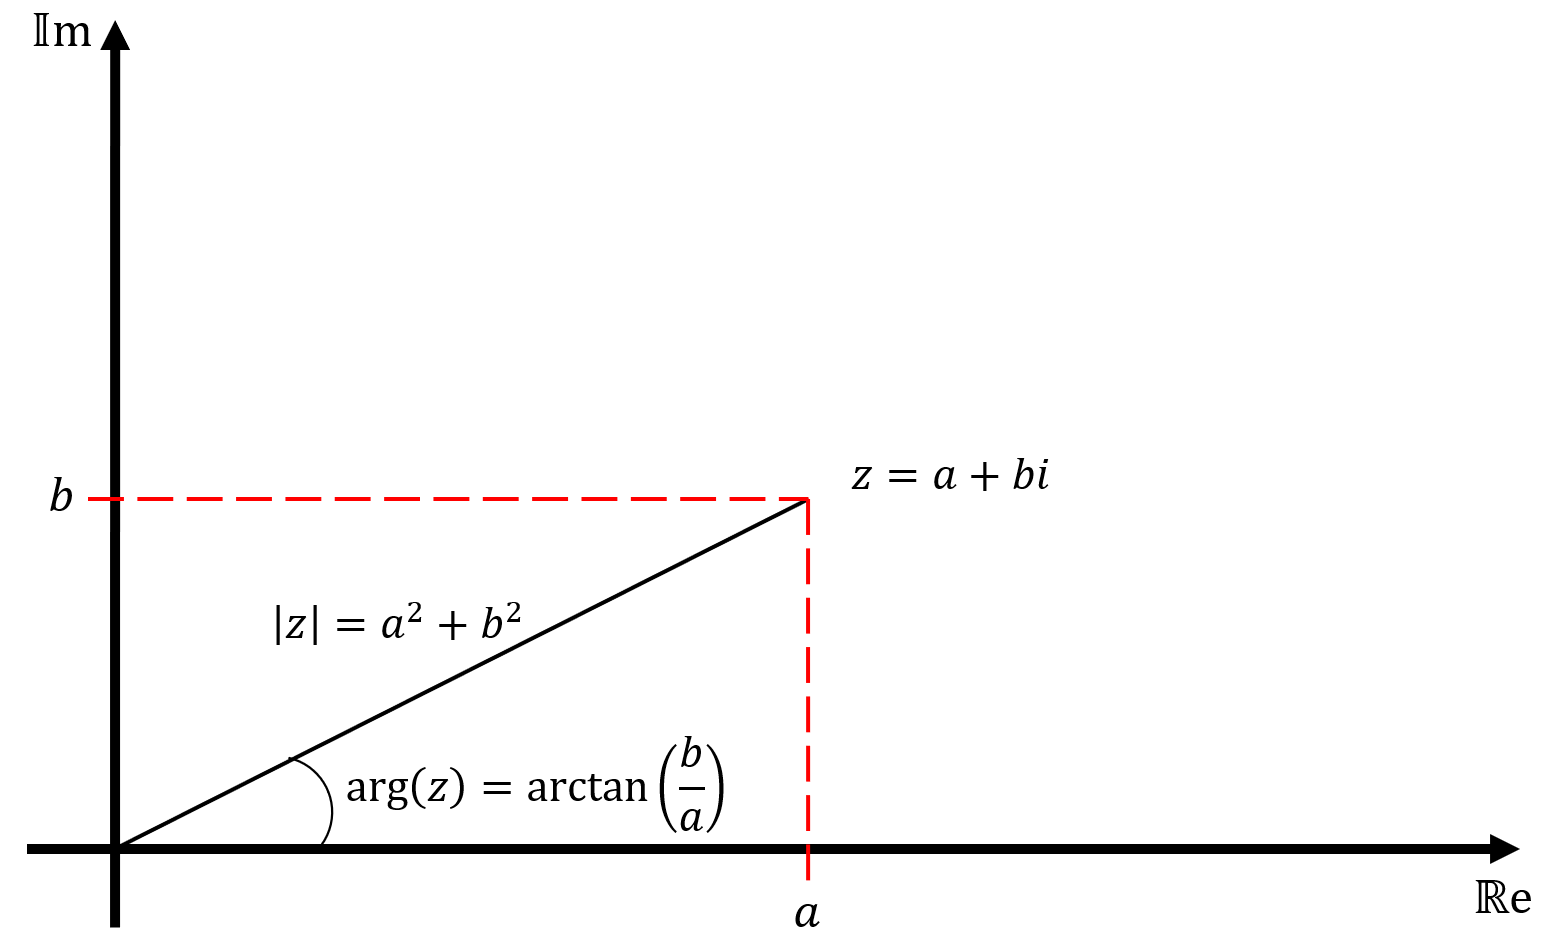
\includegraphics[width=\textwidth]{argand}}
\end{figure}
The modulus of a complex number $z=a+bi$ is given by the square root of $zz^{*}$, and is in effect the `length' of the vector that represents $z$ on an Argand diagram. The argument is the angle measured anticlockwise from the positive real axis. Of course, multiples of $2\pi$ can be added / subtracted to the argument, but the \underline{principle argument} is always in the interval $(-\pi,\pi)$.
\begin{align*}
z&=a+bi & z^{*}&=a-bi \\
\arg(z)&=\arctan\left(\frac{b}{a}\right) & \arg\left( z^{*} \right)&=\arctan\left(\frac{-b}{a}\right) \\
\end{align*}
\vspace{-1cm}
\begin{align*}
|z|&=\sqrt{zz^{*}}=\sqrt{(a+bi)(a-bi)}=\sqrt{a^{2}+\cancel{abi}-\cancel{abi}-(bi)^{2}} \\
&=\sqrt{a^{2}-b^{2}i^{2}}=\sqrt{a^{2}-b^{2}(-1)}=\sqrt{a^{2}+b^{2}}
\end{align*}

The complex number $z$ can therefore be written as
\begin{equation*}
z=r\left(\cos(\theta)+i\sin(\theta)\right)
\end{equation*}
where
\begin{align*}
r&=|z| & \theta&=\arg(z)
\end{align*}

When multiplying two complex numbers $w$ and $z$, the product, $wz$ can be evaluated fairly simply;
\begin{align*}
|wz|&=|w|\times|z| & \arg(wz)&=\arg(w)+\arg(z)
\end{align*}
\vspace{0.25cm}


\subsection{Complex number notation}
Where $z$ is a complex number with modulus $r$ and argument $\theta$;
\begin{center}
\small
\begin{tblr}{|[.75pt]|l|l||[.75pt]}
\hline[1pt]
Form & Name \\ \hline[1pt]
$z=x+iy$ & Cartesian form \\ \hline
$z=r\left(\cos(\theta)+i\sin(\theta)\right)\hspace{.5cm}$ & Modulus - argument form \\ \hline
$z=r \cis(\theta)$ & Polar form \\ \hline
$z=[r,\theta]$ & Polar form $\hspace{.5cm}$ \small{\emph{Note: Must be square brackets}} \\ \hline[.75pt]
\end{tblr}
\end{center}
\vspace{0.5cm}


\subsection{Loci in the complex plane}
\begin{itemize}
\item A Level FM AS / Year 1 \hspace{1cm} Pages 129 -- 134
\end{itemize} \par
As in section \ref{loci} on loci, a locus in the complex plane is a set of points which satisfy a certain condition. The formula booklet gives the following;
\begin{center}
\begin{tblr}{|[.75pt]|l|c||[.75pt]}
\hline[1pt]
Circles: & $|z-a|=k$ \\ \hline
Half lines: & $\arg(z-a)=\theta$ \\ \hline
Lines: & $|z-a|=|z-b|$ \\ \hline
\end{tblr}
\end{center}
Examples:
\begin{enumerate}
\item $|z-1-i|=1$
\begin{align*}
1&=\left|z-(1+i)\right| \\
1&=\left|x+iy-(1+i)\right|^{2} \\
1&=\left|(x-1)+i(y-1)\right|^{2} \\
1&=\left((x-1)+i(y-1)\right)\left((x-1)-i(y-1)\right) \\
1&=(x-1)^{2}+(y-1)^{2}
\end{align*}
\vspace{.3cm}
\item $\arg(z-2+i)=\frac{\pi}{4}$
\begin{equation*}
\arg\left(z-(2-i)\right)=\frac{\pi}{4}
\end{equation*}
The $z-(2-i)$ term maps the vector from (2-i) to $z$. This gives a half line, extending from the point representing $2-i$ in the direction with argument $\frac{\pi}{4}$
\vspace{.3cm}
\item $|z-(3+4i)|=|z-(2-5i)|$
\begin{align*}
\left|(x+iy)-(3+4i)\right|&=\left|(x+iy)-(2-5i)\right| \\
(x-3)^{2}+(y-4)^{2}&=(x-2)^{2}+(y+5)^{2} \\
\cancel{x^{2}}-6x+9 + \cancel{y^{2}}-8y+16 &= \cancel{x^{2}}-4x+4 + \cancel{y^{2}}+10y+25 \\
-2x-4&=18y \\
y&=\frac{-2x-4}{18}
\end{align*}
\end{enumerate}
\vspace{0.5cm}


\subsection{De Moivre's Theorem}
\begin{itemize}
\item A Level FM Year 2 \hspace{1cm} \phantom{AS /} Pages 25 -- 30
\item A Level FM Year 2 \hspace{1cm} \phantom{AS /} Pages 57 -- 64
\end{itemize} \par
De Moivre's Theorem states that:
\begin{equation*}
\left(\cos(\theta)+i\sin(\theta)\right)^{n}=\cos(n\theta)+i\sin(n\theta)
\end{equation*}
De Moivre's Theorem can be used to write $\cos(n\theta)$ or $\sin(n\theta)$ in terms of a sum of powers of $\cos(\theta)$ or $\sin(\theta)$ respectively.

Consider $\left(\\cos(\theta)+i\sin(\theta)\right)^{3}$. \newline \par
By De Moivre's Theorem;
\begin{equation*}
\left(\cos(\theta)+i\sin(\theta)\right)^{3}=\cos(3\theta)+i\sin(3\theta)
\end{equation*} \par
By expanding the binomial;
\scriptsize
\begin{align*}
\left(\cos(\theta)+i\sin(\theta)\right)^{3}&=\cos^{3}(\theta)+3i\cos^{2}(\theta)\sin(\theta)+3i^{2}\cos(\theta)\sin^{2}(\theta)+i^{3}\sin^{3}(\theta) \\
&=\cos^{3}(\theta)+3i\cos^{2}(\theta)\sin(\theta)-3\cos(\theta)\sin^{2}(\theta)-i\sin^{3}(\theta) \\
&=\left[ \cos^{3}(\theta)-3\cos(\theta)\sin^{2}(\theta) \right] + i\left[ 3\cos^{2}(\theta)\sin(\theta)-\sin^{3}(\theta) \right] \\
&=\left[ \cos^{3}(\theta)-3\cos(\theta)\left( 1-\cos^{2}(\theta) \right) \right] + i\left[ 3\left( 1-\cos^{2}(\theta) \right)\sin(\theta)-\sin^{3}(\theta) \right] \\
&=\left[ \cos^{3}(\theta)-3\cos(\theta)+3\cos^{3}(\theta) \right] + i\left[ 3\sin(\theta)-3\sin^{3}(\theta)-\sin^{3}(\theta) \right] \\
&=\left[ 4\cos^{3}(\theta)-3\cos(\theta)\right] + i\left[ 3\sin(\theta)-4\sin^{3}(\theta)\right] \\
\end{align*}
\normalsize

Therefore;
\begin{equation*}
\cos(3\theta)=4\cos^{3}(\theta)-3\cos(\theta)
\end{equation*}
\vspace{0.25cm}


\subsection{De Moivre's Theorem -- `backwards'}
\begin{itemize}
\item A Level FM Year 2 \hspace{1cm} \phantom{AS /} Pages 25 -- 30
\item A Level FM Year 2 \hspace{1cm} \phantom{AS /} Pages 57 -- 64
\end{itemize} \par
De Moivre's Theorem can also be used to write powers of $\cos(\theta)$ and $\sin(\theta)$ in terms of multiple angles of $\theta$.

\begin{gather*}
z=\cos(\theta)+i\sin(\theta) \\
\frac{1}{z}=\cos(-\theta)+i\sin(-\theta)=\cos(\theta)-i\sin(\theta) \\
\end{gather*}

\begin{align*}
\Rightarrow z+\frac{1}{z}&=2\cos(\theta) \\
\Rightarrow z-\frac{1}{z}&=2\sin(\theta) \\
\end{align*}
\vspace{-.75cm}
\begin{gather*}
z^{n}=\cos(n\theta)+i\sin(n\theta) \\
\frac{1}{z^{n}}=\cos(-n\theta)+i\sin(-n\theta)=\cos(n\theta)-i\sin(n\theta) \\
\end{gather*}
\vspace{-1cm}
\begin{align*}
\Rightarrow z^{n}+\frac{1}{z^{n}}&=2\cos(n\theta) \\
\Rightarrow z^{n}-\frac{1}{z^{n}}&=2\sin(n\theta) \\
\end{align*}
\vspace{0.5cm}

Now, suppose we want to find $\sin^{3}(\theta)$;
\small
\begin{flalign*}
\sin^{3}(\theta)&=\left(\frac{z-\frac{1}{z}}{2i}\right)^{3}=\frac{1}{8i^{3}}\left( z-\frac{1}{z} \right)^{3}=\frac{1}{-8i}\left( z-\frac{1}{z} \right)^{3}=\frac{i}{8}\left( z-\frac{1}{z} \right)^{3} \\
&=\frac{i}{8}\left[z^{3}-3z+\frac{3}{z}-\frac{1}{z^{3}}\right] \\
&=\frac{i}{8}\left[\left(z^{3}-\frac{1}{z^{3}}\right)-3\left(z+\frac{1}{z}\right)\right] \\
&=\frac{i}{8}\left[2i\sin(3\theta)-3\times2i\sin(\theta)\right] \\
&=-\frac{1}{4}\sin(3\theta)+\frac{3}{4}\sin(\theta)
\end{flalign*}
\normalsize
\vspace{0.25cm}

\subsection{Complex exponential form}
\begin{itemize}
\item A Level FM Year 2 \hspace{1cm} \phantom{AS /} Pages 30 -- 34
\end{itemize} \par
Also called \emph{Euler's form}, see section \ref{eulersform} for a derivation on where this comes from
\begin{equation*}
re^{i\theta}\equiv r\left(\cos(\theta)+i\sin(\theta)\right)
\end{equation*}
Where all the usual rules concerning exponents apply
\vspace{0.5cm}


\subsection{Complex roots}
\begin{itemize}
\item A Level FM Year 2 \hspace{1cm} \phantom{AS /} Pages 34 -- 38
\item A Level FM Year 2 \hspace{1cm} \phantom{AS /} Pages 45 -- 52
\end{itemize} \par
Every number, real and complex, has roots in both the real and complex plane. These can be found easily from either the modulus-argument form, or complex exponential form of the number
\begin{equation*}
z=r\left(\cos(\theta+2n\pi)+i\sin(\theta+2n\pi)\right)=re^{i(\theta+2n\pi)}
\end{equation*}
Therefore;
\begin{equation*}
\sqrt[n]{z}=\sqrt[n]{r}\left(\cos\left(\frac{\theta+2k\pi}{n}\right)+i\sin\left(\frac{\theta+2k\pi}{n}\right)\right)
\end{equation*}
For integers $n$ in the range $0\leq k \leq n-1$. \newline \par

Alternatively,
\begin{equation*}
\sqrt[n]{z}=\sqrt[n]{r}e^{i\left(\frac{\theta+2k\pi}{n}\right)}
\end{equation*}
For integers $n$ in the range $0\leq k \leq n-1$. \newline \par
\vspace{0.5cm}


\subsection{The roots of unity}
\begin{itemize}
\item A Level FM Year 2 \hspace{1cm} \phantom{AS /} Pages 39 -- 43
\end{itemize} \par
The $n$ $n^{th}$ roots of 1 form a regular polygon centred on the origin, with each point (complex root) having a modulus of 1. \newline \par

To solve equations of the form
\begin{equation*}
z^{n}=a^{n}
\end{equation*}
This can be rewritten as
\begin{equation*}
z=a\times\omega^{k}
\end{equation*}
Where
\begin{equation*}
\omega=e^{\frac{2i\pi}{n}}\hspace{1cm} \text{ and } k\in\{0,1,2,3,\dots,n-1\}
\end{equation*} \par

So the $n$ roots of $a^{n}$ can be found by writing $a^{n}$ in complex exponential form, and adding multiples of $2\pi$ to the argument. Then taking the real $n^{th}$ root of the modulus, and dividing each argument by $n$, the $n$ $n^{th}$ roots of $a^{n}$ can be found.
\vspace{0.5cm}


\subsection{The "$C+iS$" method for summing a trigonometric series}
\begin{itemize}
\item A Level FM Year 2 \hspace{1cm} \phantom{AS /} Pages 64 -- 68
\end{itemize} \par
The $C+iS$ method is useful for summing a trigonometric series involving functions of multiple angles. This is best illustrated by an example.

\begin{align*}
C&=\cos(\theta)+\frac{1}{2}\cos(3\theta)+\frac{1}{4}\cos(5\theta)+\frac{1}{8}\cos(7\theta)+\cdots \\
S&=\sin(\theta)+\frac{1}{2}\sin(3\theta)+\frac{1}{4}\sin(5\theta)+\frac{1}{8}\sin(7\theta)+\cdots
\end{align*}

\begin{flalign*}
&w=C+iS & \left[\text{Plan: Find $w$, then take $C=\mathfrak{Re}(w)$}\right]&
\end{flalign*}
\begin{flalign*}
w=&(\cos(\theta)+i\sin(\theta))+\frac{1}{2}(\cos(3\theta)+i\sin(3\theta)) && \\ &\hspace{2cm}+\frac{1}{4}(\cos(5\theta)+i\sin(5\theta))+\frac{1}{8}(\cos(7\theta)+i\sin(7\theta))+\cdots \\
& && \\
=&e^{i\theta}+\frac{1}{2}e^{3i\theta}+\frac{1}{4}e^{5i\theta}+\frac{1}{8}e^{7i\theta}+\cdots \\
\end{flalign*}
This is a geometric series, with a first term of $e^{i\theta}$, and common ratio of $\frac{1}{2}e^{2i\theta}$. Therefore;
\begin{flalign*}
w&=\frac{e^{i\theta}}{1-\frac{1}{2}e^{2i\theta}}=\frac{2e^{i\theta}}{2-e^{2i\theta}}=\frac{2e^{i\theta}\left(2-e^{-2i\theta}\right)}{\left(2-e^{2i\theta}\right)\left(2-e^{-2i\theta}\right)} && \\
&=\frac{4e^{i\theta}-2e^{-i\theta}}{4+1-2\left(e^{i2\theta}+e^{-i2\theta}\right)} \\
&=\frac{4\cos(\theta)+4i\sin(\theta)-2\cos(\theta)+2i\sin(\theta)}{5-4\cos(2\theta)} \\
&=\frac{2\cos(\theta)}{5-4\cos(2\theta)} +i\frac{6\sin(\theta)}{5-4\cos(2\theta)} \hspace{2.5cm} \text{and }w=C+iS \\
\end{flalign*}
Therefore
\begin{align*}
C&=\frac{2\cos(\theta)}{5-4\cos(2\theta)} & S=\frac{6\sin(\theta)}{5-4\cos(2\theta)}
\end{align*}
\vspace{0.5cm}

\end{document}